\documentclass[a4paper]{arrowhead}

\usepackage[yyyymmdd]{datetime}
\usepackage{etoolbox}
\usepackage[utf8]{inputenc}
\usepackage{multirow}

\renewcommand{\dateseparator}{-}

\setlength{\parskip}{1em}

%% Special references
\newcommand{\fref}[1]{{\textcolor{ArrowheadBlue}{\hyperref[sec:functions:#1]{#1}}}}
\newcommand{\mref}[1]{{\textcolor{ArrowheadPurple}{\hyperref[sec:model:#1]{#1}}}}
\newcommand{\pdef}[1]{{\textcolor{ArrowheadGrey}{#1\label{sec:model:primitives:#1}\label{sec:model:primitives:#1s}\label{sec:model:primitives:#1es}}}}
\newcommand{\pref}[1]{{\textcolor{ArrowheadGrey}{\hyperref[sec:model:primitives:#1]{#1}}}}

\newrobustcmd\fsubsection[3]{
  \addtocounter{subsection}{1}
  \addcontentsline{toc}{subsection}{\protect\numberline{\thesubsection}function \textcolor{ArrowheadBlue}{#1}}
  \renewcommand*{\do}[1]{\rref{##1},\ }
  \subsection*{
    \thesubsection\quad
    operation
    \textcolor{ArrowheadBlue}{#1}
    (\notblank{#2}{\mref{#2}}{})
    \notblank{#3}{: \mref{#3}}{}
  }
  \label{sec:functions:#1}
}
\newrobustcmd\msubsection[2]{
  \addtocounter{subsection}{1}
  \addcontentsline{toc}{subsection}{\protect\numberline{\thesubsection}#1 \textcolor{ArrowheadPurple}{#2}}
  \subsection*{\thesubsection\quad#1 \textcolor{ArrowheadPurple}{#2}}
  \label{sec:model:#2} \label{sec:model:#2s} \label{sec:model:#2es}
}
%%

\begin{document}

%% Arrowhead Document Properties
\ArrowheadTitle{XXX} % XXX = ServiceName 
\ArrowheadServiceID{ID} % ID name of service
\ArrowheadType{Service Description}
\ArrowheadTypeShort{SD}
\ArrowheadVersion{X.Y.Z} % Arrowhead version X.Y.Z, e..g. 4.4.1
\ArrowheadDate{\today}
\ArrowheadAuthor{Doument author} % Corresponding author e.g. Jerker Delsing
\ArrowheadStatus{RELEASE} % e..g. RELEASE, RELEASE CONDIDATE, PROTOTYPE
\ArrowheadContact{xx@yy.xx} % Email of corresponding author
\ArrowheadFooter{\href{www.arrowhead.eu}{www.arrowhead.eu}}
\ArrowheadSetup
%%

%% Front Page
\begin{center}
  \vspace*{1cm}
  \huge{\arrowtitle}

  \vspace*{0.2cm}
  \LARGE{\arrowtype}
  \vspace*{1cm}

  %\Large{Service ID: \textit{"\arrowid"}}
  \vspace*{\fill}

  % Front Page Image
  %\includegraphics{figures/TODO}

  \vspace*{1cm}
  \vspace*{\fill}

  % Front Page Abstract
  \begin{abstract}
    This is the template for Service Description (SD document)
    according to the Eclipse Arrowhead documentation structure. 
  \end{abstract}

  \vspace*{1cm}

%   \scriptsize
%   \begin{tabularx}{\textwidth}{l X}
%     \raisebox{-0.5\height}{
\includegraphics[width=2cm]{figures/artemis_logo}} & {ARTEMIS Innovation Pilot Project: Arrowhead\newline
%     THEME [SP1-JTI-ARTEMIS-2012-AIPP4 SP1-JTI-ARTEMIS-2012-AIPP6]\newline
%     [Production and Energy System Automation Intelligent-Built environment and urban infrastructure for sustainable and friendly cities]}
%   \end{tabularx}
%   \vspace*{-0.2cm}
 \end{center}

\newpage
%%

%% Table of Contents
\tableofcontents
\newpage
%%

\section{Overview}
\label{sec:overview}
\color{red}
This document describes the [XX] service, which is enables [brief description of service capabilities]. 

The rest of this document is organized as follows.
In Section \ref{sec:functions}, we describe the abstract message functions provided by the service.
In Section \ref{sec:model}, we end the document by presenting the data types used by the mentioned functions.
\color{black}

\newpage

\subsection{Significant Prior Art}

\color{red} Describe significant prior art which provides the
foundation for the service - May be omitted for simple services \color{black}  

\subsection{How This Service Is Meant to Be Used}
\color{red} Describe intended usage of the service \color{black}  


\subsection{Important Delimitations}
\label{sec:delimitations}

\color{red} Provide delimitations of the provided service \color{black}  



\newpage

\section{Service Interface}
\label{sec:functions}

\color{red}
This section describes the interfaces to the [XX] service.
In particular, each subsection names an abstract operation, an input type and an output type, in that order.
The input type is named inside parentheses, while the output type is preceded by a colon.
Input and output types are only denoted when accepted or returned, respectively, by the interface in question.

All abstract data types named in this section are defined in Section \ref{sec:model}.
\color{black}

\begin{figure}[h!]
  \centering
  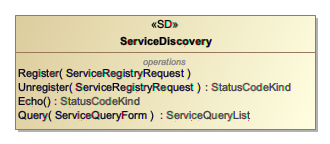
\includegraphics[width=10cm]{figures/ServiceDiscovery_SD}
  \caption{\color{red} EXAMPLE: SysML block description diagram of the ServiceDiscovery and
    its interface \color{black}}
  \label{fig:SD}
\end{figure}

The following interface operations are available.

\fsubsection{AA}{aa}{response}

\color{red} 
The AA operation is used to ..... The services will contain various
metadata as well as a physical endpoint. The various parameters are
representing the necessary service input information.
\color{black}

\fsubsection{BB}{bb}{response}

\color{red} 
The BB operation is used to .... 
\color{black}

\fsubsection{CC}{cc}{Response}

\color{red} 
The CC operation enable ......
\color{black}

\fsubsection{Echo}{}{StatusCodeKind}

\color{red} 
The Echo operation provides an is alive response from the XX service.
\color{black}

\newpage

\section{Information Model}
\label{sec:model}

\color{red} 
Here, all data objects that can be part something the XX Service
provides to the hosting System are listed in alphabetic order.
Note that each subsection, which describes one type of object, begins with the \textit{struct} keyword, which is used to denote a collection of named fields, each with its own data type.
As a complement to the explicitly defined types in this section, there is also a list of implicit primitive types in Section \ref{sec:model:primitives}, which are used to represent things like hashes and identifiers.
\color{black}

An overview of the data object types is illustrated in Figure \ref{fig:model_overview}.

\begin{figure}[ht!]
  \centering
  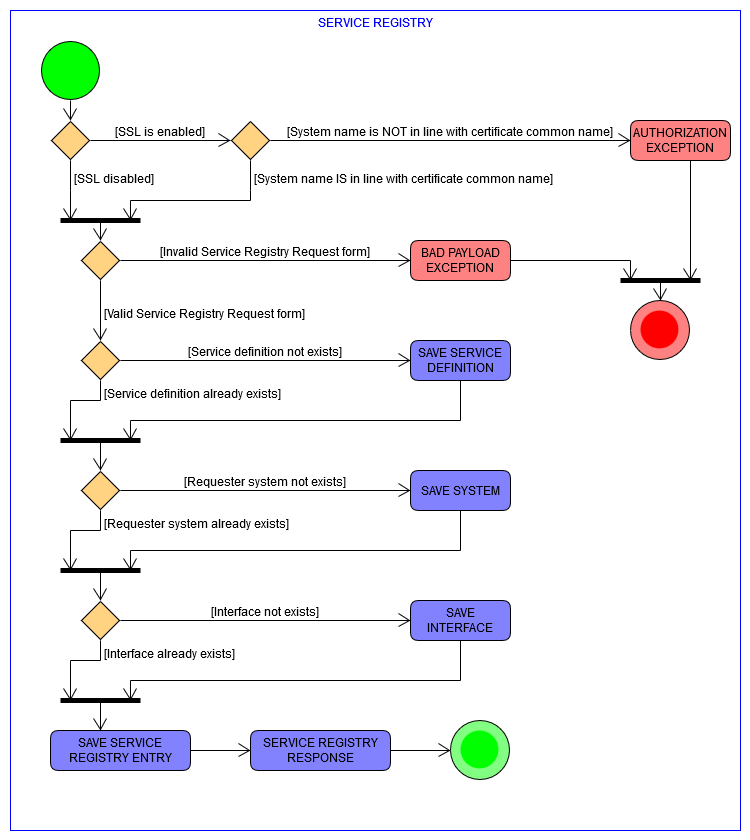
\includegraphics[width=\textwidth]{figures/post_service_registry_register_activity_uml}
  \caption{\color{red} EXAMPLE:
    Information model as a UML activity diagram.
    Describes the process of service registration.
    \color{black}
  }
  \label{fig:model_overview}
\end{figure}

\msubsection{struct}{ServiceRegistryRequest}

\color{red} 
 EXAMPLE: This structure is used to register a service offering into the Service Registry.
\color{black}
 
\begin{table}[ht!]
\begin{tabularx}{\textwidth}{| p{4.25cm} | p{3.5cm} | X |} \hline
\rowcolor{gray!33} Field & Type      & Description \\ \hline
endofValidity                 & \pref{DateTime} & Service is available until this UTC timestamp. \\ \hline
interfaces                   & \pref{Array}$<$\pref{Interface}$>$     & List of interfaces the service supports. \\ \hline
metadata                  & \pref{Metadata}     & Metadata \\ \hline
providerSystem                    & \pref{Name} & Name of the provider system. \\ \hline
secure                   &\pref{SecureType}  & Type of security the service uses. \\ \hline
serviceDefinition         &\pref{Name}        & Service Definition. \\ \hline
serviceUri                &\pref{URI}         & URI of the service. \\ \hline
version                   &\pref{Version}     & Version of the service. \\ \hline
\end{tabularx}
\end{table}

\begin{figure}[ht!]
  \centering
  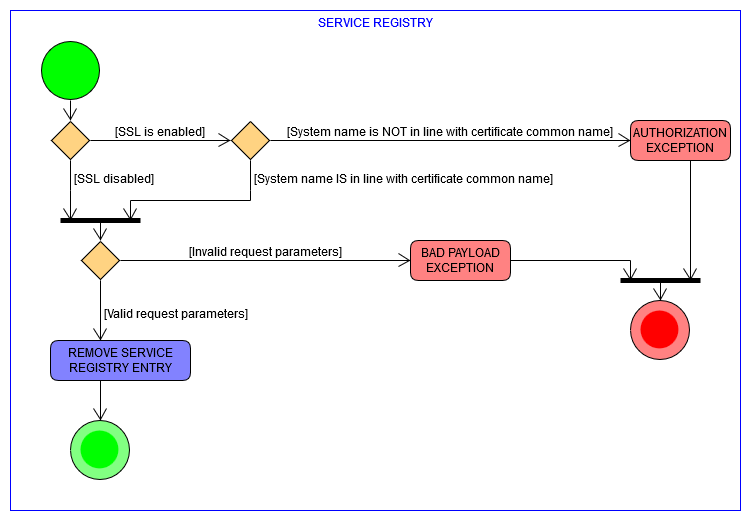
\includegraphics[width=\textwidth]{figures/delete_service_registry_unregister_activity_uml.png}
  \caption{\color{red}  EXAMPLE:
    Information model as a UML activity diagram.
    Describes the process of service unregistration.
    \color{black}
  }
  \label{fig:unregister_overview}
\end{figure}

\msubsection{struct}{ServiceRegistryUnregisterRequest}

\color{red} 
EXAMPLE: This structure is used to register a service offering into
the Service Registry. Please also refer to the activity diagram in
Figure \ref{fig:unregister_overview} \color{black}

\begin{table}[ht!]
\begin{tabularx}{\textwidth}{| p{4.25cm} | p{3.5cm} | X |} \hline
\rowcolor{gray!33} Field & Type      & Description \\ \hline
address                 & \pref{Address} & Address of the provider systems. \\ \hline
port                   & \pref{PortNumber}     & Port of the provider system. \\ \hline
system\_name                  & \pref{Name}     & System name of the provider system \\ \hline
service\_definition                    & \pref{Name} & Service Definition of the unregistered service. \\ \hline
\end{tabularx}
\end{table}

\begin{figure}[ht!]
  \centering
  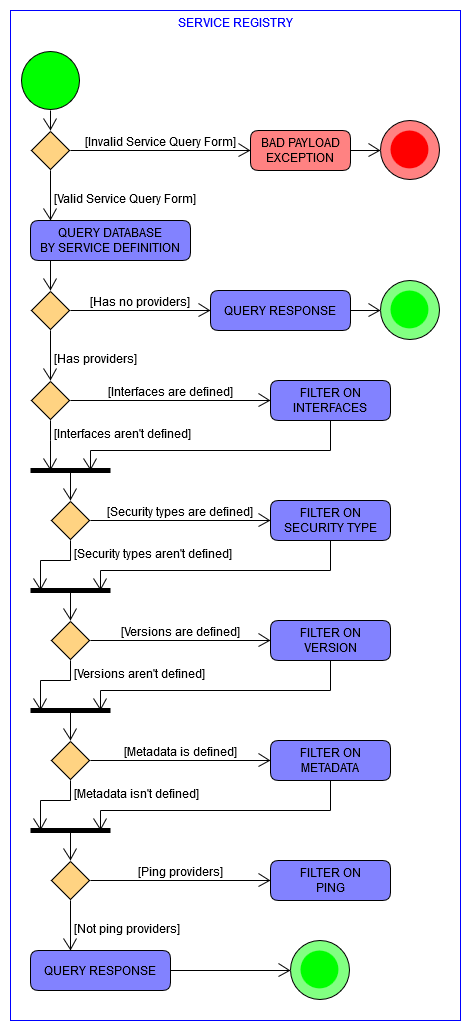
\includegraphics[width=\textwidth,height=0.9\textheight,keepaspectratio]{figures/post_service_registry_query_activity_uml.png}
  \caption{\color{red}  EXAMPLE:
    Information model as a UML activity diagram. Describes the process
    of service querying.
    \color{black}
  }
  \label{fig:query_overview}
\end{figure}

\msubsection{struct}{ServiceQueryForm}

\color{red} 
EXAMPLE: This structure is used to query service offering registered in
the Service Registry. Please also refer to the activity diagram in
Figure \ref{fig:query_overview} \color{black}

\begin{table}[ht!]
\begin{tabularx}{\textwidth}{| p{5cm} | p{3.5cm} | X |} \hline
\rowcolor{gray!33} Object Field & Value Type      & Description \\ \hline
"interfaceRequirements"                   & \pref{Array}$<$\pref{Interface}$>$     & List of the required interfaces. \\ \hline
"maxVersionRequirement"                & \pref{Version}     & Maximum version. \\ \hline
"minVersionRequirement"                & \pref{Version}     & Minimum version. \\ \hline
"metadataRequirements"                  & \pref{Metadata}     & Metadata. \\ \hline
"pingProviders".                    & \pref{Boolean} & Checks the availability of the providers if true \\ \hline
"securityRequirements"                    &\pref{Name}  & Type of security. \\ \hline
"serviceDefinitionRequirement"         &\pref{Name}        & Service Definition. \\ \hline
"versionRequirement"                   &\pref{Version}     & Version of the service. \\ \hline
\end{tabularx}
\end{table}


\subsection{Primitives}
\label{sec:model:primitives}

Types and structures mentioned throughout this document that are assumed to be available to implementations of this service.
The concrete interpretations of each of these types and structures must be provided by any IDD document claiming to implement this service.


\begin{table}[ht!]
\begin{tabularx}{\textwidth}{| p{3cm} | X |} \hline
\rowcolor{gray!33} Type & Description \\ \hline
\pdef{Address}          & A string representation of the address \\ \hline
\pdef{Boolean}          & One out of \texttt{true} or \texttt{false}. \\ \hline
\pdef{Interface}        & Any suitable type chosen by the implementor of the service. \\ \hline
\pdef{DateTime}         & Pinpoints a specific moment in time. \\ \hline
\pdef{List}$<$A$>$      & An \textit{array} of a known number of items, each having type A. \\ \hline
\pdef{Name}             & A string identifier that is intended to be both human and machine-readable. \\ \hline
\pdef{PortNumber}       & Decimal number in the range of 0-65535 \\ \hline
\pdef{Version}         & Specifies a service version. \\ \hline
\end{tabularx}
\end{table}

\newpage

\bibliographystyle{IEEEtran}
\bibliography{bibliography}

\newpage

\section{Revision History}
\subsection{Amendments}

\noindent\begin{tabularx}{\textwidth}{| p{1cm} | p{3cm} | p{2cm} | X | p{4cm} |} \hline
\rowcolor{gray!33} No. & Date & Version & Subject of Amendments & Author \\ \hline

1 & 2020-12-05 & \arrowversion & & Tanyi Szvetlin \\ \hline
2 & 2021-07-14 & \arrowversion & Minor updates & Jerker Delsing \\ \hline
3 & 2022-01-10 & \arrowversion & Minor updates & Jerker Delsing \\ \hline
\end{tabularx}

\subsection{Quality Assurance}

\noindent\begin{tabularx}{\textwidth}{| p{1cm} | p{3cm} | p{2cm} | X |} \hline
\rowcolor{gray!33} No. & Date & Version & Approved by \\ \hline

1 & 2022-01-10 & \arrowversion  &  \\ \hline

\end{tabularx}

\end{document}